\documentclass[11pt]{article}
\usepackage[T1]{fontenc}
\usepackage[utf8]{inputenc}
\usepackage{lmodern}
\usepackage{amsmath}
\usepackage{graphicx}
\usepackage{booktabs}
\usepackage{tabularx}
\usepackage{array}
\usepackage{textcomp}
\usepackage[hidelinks]{hyperref}
\newcommand{\EG}{\textsc{EventGuard}}
\newcommand{\IO}{\textsc{Importance-Only}}
\newcommand{\LO}{\textsc{Link-Only}}
\newcommand{\UB}{\textsc{Uniform-Budget}}
\newcommand{\RB}{\textsc{Random-Budget}}
\newcommand{\Fone}{\textsc{Fixed-1}}
\newcommand{\Ftwo}{\textsc{Fixed-2}}
\newcommand{\Fthree}{\textsc{Fixed-3}}
\title{Disentangling Event Importance, Transmission Budget, and Link-State Adaptation under Software-Injected Loss}
\author{Author Name\\Affiliation\\\texttt{Email}}
\date{}
\begin{document}
\maketitle

\begin{abstract}
Periodic IoT traffic includes events whose loss matters more than routine-sample loss, but uniform redundancy ignores event value. We study frozen \EG{}-v1, which combines predicted event importance with first-copy ACK-based link state to select up to three proactive DATA copies. The original evaluation comprises 8,000 host runs, 11,000 host-only sensitivity runs, and a post-hoc balanced analysis of 96 completed ESP32-S3/E220-400T22D runs; all 96 passed offline audit. At an exact DATA-copy budget, \EG{} directed more copies to CRITICAL samples than event-blind controls and gained modest CRITICAL delivery in some \texttt{RANDOM\_COPY} conditions, but not under constructed \texttt{BURST\_SAMPLE} erasure. Correctly classified CRITICAL samples already receive the three-copy cap in every link state, explaining their identical delivery under \EG{} and \IO{}. \EG{} showed higher IMPORTANT and overall delivery than the lower-budget \IO{} rule under \texttt{RANDOM\_COPY}, but this comparison changes both link-state use and copy budget. A separate \textbf{post-hoc, host-only, exploratory} 500-run diagnostic introduced \textsc{Importance-Matched-Budget} (IMB), a link-blind allocator with the same predicted importance, seed-specific \EG{} DATA-copy budget, trace, and canonical loss calendar. IMB reproduced most of the earlier IMPORTANT/overall uplift over \IO{}; \EG{}-minus-IMB differences were mixed and near zero at 20\% and 30\% loss. This diagnostic was designed after inspecting v1 results, was not preregistered, and is neither part of the original 8,000-run matrix nor frozen \texttt{v1.0.0}. The evidence supports importance-aware allocation and added budget while showing no consistent incremental placement advantage for the evaluated link response against this specific counterfactual under deterministic software-injected loss. It does not establish performance under measured RF fading.

\end{abstract}

\noindent\textbf{Keywords:} constrained IoT communication; event importance; proactive redundancy; exact-budget evaluation; ESP32-S3; Sub-GHz radio.

\section{Introduction}\label{sec:introduction}

Periodic sensing is often evaluated by average packet delivery, which weighs a routine observation and an urgent event equally. In a constrained IoT link, extra copies consume communication capacity; their value depends on which events receive them. \EG{} combines predicted event importance with recent first-copy ACK outcomes, but three factors can be conflated: importance-aware allocation, the number of DATA copies spent, and placement driven by estimated link state. We ask four questions: Does importance improve CRITICAL delivery at equal budget? How much of \EG{}'s secondary-delivery gain follows from extra transmission budget? At the same budget and predicted importance, does link-state-aware placement improve on a link-blind allocator? How does programmed loss structure affect these comparisons?

In the original comparison, \EG{} and \IO{} differ in both link-state use and transmission budget. It cannot by itself isolate link-state-aware placement. This is especially important because frozen v1 already gives correctly classified CRITICAL samples three copies in every state: link adaptation has no remaining copy-allocation action for the original primary KPI. The mechanism still has action space for IMPORTANT and NORMAL samples, but observing their higher delivery against a lower-budget rule does not identify why they improved. We therefore use exact-budget event-blind controls for the importance question and a separately protocolized, \textbf{post-hoc host-only IMB diagnostic} for the question of budget and placement. The IMB design was fixed after inspecting frozen v1 results but before generating its outcomes.

The study retains the frozen 8,000-run host matrix, 11,000 sensitivity runs, and execution through a two-device ESP32-S3/E220 DATA/ACK path. The planned 160-run device experiment was interrupted by an unresolved receive-path stall; its selected 96-run subset comprises the earliest six contiguous seeds with complete four-strategy/four-condition coverage. Selection used execution order and completeness, not comparative outcome. Its \(n=6\) sample size was not preregistered, so device results are descriptive. The additional IMB runs were performed only on the host and are not part of the frozen \texttt{v1.0.0} study.

This paper contributes:
\begin{enumerate}
\item A frozen, interpretable event-importance redundancy policy and exact-budget event-blind controls that test where a fixed transmission budget is spent.
\item Component ablations showing structural saturation of correctly classified CRITICAL samples at the three-copy cap.
\item A post-hoc exact-budget IMB diagnostic: a link-blind, importance-aware allocator reproduces most of the earlier IMPORTANT/overall uplift over \IO{}, with no consistent incremental advantage for \EG{}'s link-state-aware placement under deterministic \texttt{RANDOM\_COPY} injection.
\item Reproducible host and device-path evaluation with preserved negative results, an unresolved later hardware anomaly, raw records, and provenance.
\end{enumerate}

The bounded conclusion is that importance information and additional copies explain the main observed benefits under these programmed-loss conditions. The IMB contrast assesses one specific link-blind placement rule, not every possible allocator or a measured RF channel.

\section{Related Work}\label{sec:related-work}

\subsection{LPWAN reliability and replication}\label{sec:lpwan-reliability-and-replication}

LoRaWAN specifies confirmed uplink traffic and associated downlink behavior \cite{lorawan104}, but ACKs and retransmissions incur capacity and duty-cycle costs. Capuzzo \emph{et al.} analyze pitfalls of confirmed traffic \cite{capuzzo2018confirmed}, while Adelantado \emph{et al.} describe broader LoRaWAN operating limits \cite{adelantado2017limits} and Magrin \emph{et al.} examine how parameter choices, including confirmed-traffic settings, affect system performance \cite{magrin2020lorawan}. These studies motivate cost-aware reliability evaluation; they do not provide a direct protocol baseline because our E220 devices use a custom application protocol rather than LoRaWAN. Hybrid coded replication in LoRa networks explicitly trades redundancy against reliability \cite{santana2020hybrid}. Our proactive copies are uncoded and deliberately simple, making the allocation rule and its cost visible. The constructed \texttt{BURST\_SAMPLE} model further tests the limit of repeating copies within a single logical sample; it is not a measurement of LoRaWAN or RF burst errors.

\subsection{Link-quality-aware adaptation}\label{sec:link-quality-aware-adaptation}

Link estimation in sensor networks has long combined observations across protocol layers, including packet and ACK outcomes \cite{fonseca2007fourbit}. Srinivasan \emph{et al.} show that wireless losses can be bursty, so a single mean delivery rate need not characterize temporal behavior \cite{srinivasan2008beta}. LoRaWAN adaptive-data-rate work uses link observations to adjust radio parameters and studies convergence under changing conditions \cite{finnegan2020adr}. Our estimator is narrower: it uses accepted first-copy ACK history to select a bounded number of application DATA copies, without changing physical-layer settings. These references support examining when history predicts future outcomes; they do not establish that this estimator captures time-varying E220 channel quality under the software-injected losses studied here.

\subsection{Importance-aware and event-aware communication}\label{sec:importance-aware-and-event-aware-communication}

Data-importance-aware retransmission for edge learning allocates radio resources according to training-sample utility as well as channel conditions \cite{liu2021dataimportance}. Importance-aware user scheduling likewise incorporates learning-task value into wireless acquisition \cite{liu2021scheduling}. Broader semantic and task-oriented communication research asks how transmission should reflect the receiver's intended task rather than treating every bit as equally valuable \cite{lan2021semantic}. Event-triggered sensor-network transmission has also been studied to reduce communication devoted to measurements that do not warrant an update \cite{ge2019eventtriggered}. These works motivate application-aware prioritization, but their objectives, importance measures, and actions differ from ours: \EG{} uses a fixed synthetic sensor-event classifier and proactive whole-frame replication, not model-uncertainty ARQ, semantic encoding, or event-triggered omission of routine samples. We claim neither field validation for the four sensor modalities nor priority over those methods.

\subsection{Position of this study}\label{sec:position-of-this-study}

The methodological question here is narrower than a general claim for adaptive LPWAN reliability. We separate predicted event importance from ACK-history link response, compare allocation at an exact DATA-copy budget, and test both independent copy erasures and common-mode sample erasures. The real-device study checks execution of this frozen logic and its post-reception injection path on one E220 pair. It cannot adjudicate the relative performance of the cited methods on their own protocols, workloads, or measured radio channels.

\section{System Model and Problem Formulation}\label{sec:system-model}

A \textbf{logical sample} \(i\) is one timestamped vector \(x_i\) of temperature, humidity, light, and soil-moisture values. The synthetic trace generator also assigns a ground-truth event category \(g_i\in\{N,I,C\}\) from phase semantics and hazard criteria; the on-node classifier does not read \(g_i\). It predicts \(\hat g_i\) from sensor values and its prior state. A \textbf{physical DATA copy} is one transmitted frame for sample \(i\), identified by the same logical sequence number and a copy index. The gateway validates its CRC, applies any planned receive-side DATA erasure, and deduplicates copies before counting a logical delivery. Accepted DATA elicits an ACK frame. An ACK may be physically received yet rejected by a planned application-layer ACK erasure; only an accepted first-copy ACK enters the link estimator. A scheduled set of copies is proactive redundancy, not an ACK-timeout retransmission.

Let \(r_i\in\{1,2,3\}\) be the selected number of DATA copies and \(Y_i=1\) when at least one copy of sample \(i\) is accepted after the specified injected-loss path; otherwise \(Y_i=0\). Let \(\mathcal C=\{i:g_i=C\}\) and \(\mathcal I=\{i:g_i=I\}\) for a trace of \(N\) logical samples. The delivery metrics and DATA-copy budget are

\begin{equation}\label{eq:critical-delivery}
R_C=\frac{\sum_{i\in \mathcal C}Y_i}{|\mathcal C|},\quad R_I=\frac{\sum_{i\in \mathcal I}Y_i}{|\mathcal I|},\quad R_{\mathrm{all}}=\frac{1}{N}\sum_{i=1}^{N}Y_i,\quad B=\sum_i r_i.
\end{equation}

\(R_C\) is the original primary KPI. \(R_I\) and \(R_{\mathrm{all}}\) are exploratory secondary delivery KPIs in the post-hoc diagnostic. At a fixed DATA-copy budget \(B\), the motivating allocation problem is to improve \(R_C\), while tracking physical DATA copies, DATA/ACK bytes, and other communication costs. \EG{} is a deterministic heuristic for this problem, not a claimed optimizer. Equal \(B\) does \textbf{not} imply equal total bytes because delivered copies generate ACK activity. Matching additionally holds the seed-specific trace and canonical DATA/ACK loss calendar fixed. The first-copy calendar is shared across strategies; effective loss over attempted copies can differ when strategies select different copy opportunities.

\begin{figure}[t]
\centering
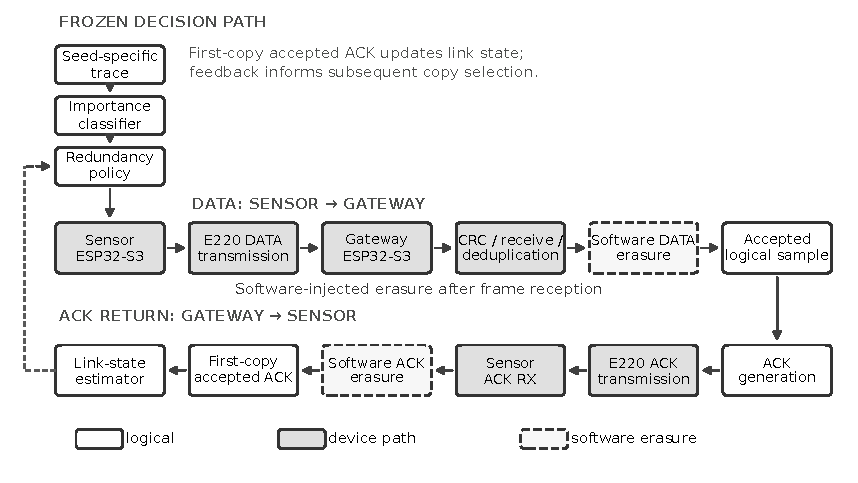
\includegraphics[width=\linewidth]{figures/fig1_system_architecture.pdf}
\caption{Frozen v1 device and decision paths. The seed-specific trace drives classification and copy selection on the Sensor ESP32-S3. The main DATA path runs left to right from Sensor through E220 and Gateway reception to the accepted logical sample; ACK follows the return path. Dashed boxes mark software erasures applied after frame reception. Only accepted first-copy ACK outcomes update the link-state estimator and inform subsequent copy selection. Configured loss is not a measured RF packet-error rate.}
\label{fig:system}
\end{figure}

\section{EventGuard Design}\label{sec:design}

\subsection{Importance estimation}\label{sec:importance-estimation}

The frozen classifier uses normalized inter-sample change, deviation from a normal-state baseline, rate of change, simultaneous change across channels, and event persistence. The four normalization scales are 0.5 \textdegree{}C, 5 humidity points, 100 lux, and 8 soil-moisture points. A directional risk rule identifies severe soil-moisture decline or combined elevated temperature/humidity. The IMPORTANT score threshold is 0.85 and the CRITICAL directional-risk threshold is 3.0. Normal observations update the baseline with coefficient 0.06. Exact equations and evaluation hashes are preserved in the frozen algorithm specification. The synthetic-trace classifier's CRITICAL precision (0.8125) and recall (1.0000) describe this constructed benchmark; they are not field accuracy estimates.

\subsection{First-copy link-state estimation}\label{sec:first-copy-link-state-estimation}

The estimator records accepted-ACK outcomes for the \textbf{first} DATA copy of each logical sample, avoiding the strategy-dependent observation count that would result from including every extra copy. A 12-observation sliding window gives a first-copy success ratio. State is BAD for three consecutive first-copy failures or a ratio below 0.50; otherwise DEGRADED below 0.80; otherwise GOOD. The initial no-observation ratio is one. Physical ACK reception, injected ACK drop, and accepted ACK remain separate records.

\subsection{Redundancy allocation}\label{sec:redundancy-allocation}

Table~\ref{tab:parameters} records the frozen parameters. The base mapping assigns NORMAL/IMPORTANT/CRITICAL to one/two/three copies on a GOOD link. DEGRADED adds one base copy, clipped to the three-copy cap. BAD adds two only to IMPORTANT or CRITICAL, likewise clipped; NORMAL remains at one. The complete decision map is shown in Fig.~\ref{fig:policy-matrix}. All selected copies are transmitted irrespective of an earlier ACK.

\begin{table}[t]
\centering
\small
\caption{Frozen v1 parameters relevant to the primary evaluation. Study matrix fields are taken from the frozen evaluation manifest; the root default configuration also contains older pilot-matrix defaults, discussed in Section~\ref{sec:versioned-configuration}.}
\label{tab:parameters}
\begin{tabularx}{\linewidth}{@{}p{0.52\linewidth}X@{}}
\toprule
Parameter & Value \\
\midrule
Trace & 9 phases \ensuremath{\times} 6 samples = 54 samples per seed \\
Inter-sample interval & 10 s \\
IMPORTANT / CRITICAL threshold & 0.85 / 3.0 \\
Importance baseline coefficient & 0.06 \\
Link window & 12 first-copy outcomes \\
DEGRADED / BAD ratio thresholds & 0.80 / 0.50 \\
BAD consecutive first-copy failures & 3 \\
Maximum copies per sample & 3 \\
ACK wait timeout & 1,000 ms \\
DATA / ACK frame length & 26 / 13 bytes \\
E220 UART rate & 9,600 bit/s \\
\bottomrule
\end{tabularx}
\end{table}

\begin{figure}[t]
\centering
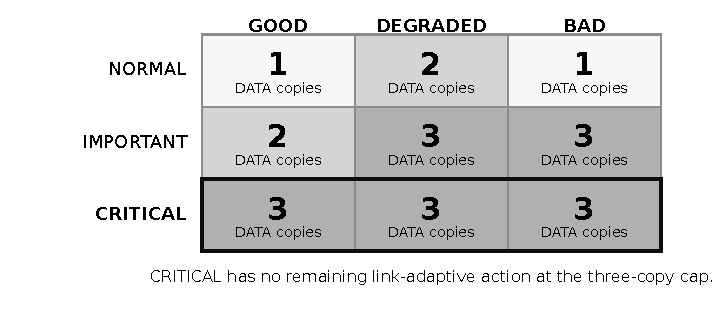
\includegraphics[width=\linewidth]{figures/fig2_policy_matrix.pdf}
\caption{Frozen v1 redundancy decision matrix. Cell values are proactive DATA copies per logical sample, indexed by predicted importance and pre-sample link state. The CRITICAL row remains 3/3/3 at the frozen three-copy cap; this is policy structure, not an empirical estimate.}
\label{fig:policy-matrix}
\end{figure}

\subsection{Structural implication}\label{sec:structural-implication}

For a \textbf{correctly classified} CRITICAL sample, \(r_i=3\) even when the link is GOOD. Because \(r_i\leq3\), no DEGRADED or BAD transition can raise its redundancy. This is a constraint of frozen v1, not an empirical estimate. Link adaptation can alter NORMAL and IMPORTANT copy counts, and might matter for a misclassified critical event; on the evaluated synthetic trace, however, CRITICAL recall was 1.0000. A critical-delivery advantage over \IO{} therefore had little policy action space in this experiment.

\section{Baselines and Budget Fairness}\label{sec:baselines}

Table~\ref{tab:strategies} separates diagnostic ablations from exact-budget comparisons. The fixed rules, \Fone{}, \Ftwo{}, and \Fthree{}, send a constant one, two, or three copies. \IO{} applies the frozen 1/2/3 importance rule without link adaptation. \LO{} applies 1/2/3 copies for GOOD, DEGRADED, and BAD, respectively, without importance. Neither fixed baselines nor component ablations are equal-cost by construction, so their delivery contrasts must be read alongside cost.

For each matched model/rate/seed/trace, the \EG{} reference determines \(B\). \UB{} first assigns one copy to each sample, then allocates remaining copies by a fixed round-robin order up to the cap. \RB{} allocates the extras by a seeded hash ordering. Their decisions may use the sample index, fixed budget, and allocation seed, but not ground truth, predicted importance, classifier score, or sensor values. The hardware budget is computed from the frozen host reference before strategy execution, allowing a seeded, interleaved execution order rather than always running \EG{} first. Actual DATA-copy totals are checked against the reference budget.

\begin{table}[t]
\centering
\footnotesize
\caption{Evaluated strategies and comparison roles. All eight appear in the host matrix; the four marked hardware appear in the final 96-run set.}
\label{tab:strategies}
\begin{tabularx}{\linewidth}{@{}p{0.23\linewidth}>{\raggedright\arraybackslash}p{0.31\linewidth}>{\raggedright\arraybackslash}Xc@{}}
\toprule
Strategy & Copy rule & Role & Hardware set \\
\midrule
\Fone{} & One per sample & Minimal fixed-copy comparison & No \\
\Ftwo{} & Two per sample & Fixed-copy comparison & No \\
\Fthree{} & Three per sample & Maximum fixed-copy comparison & No \\
\IO{} & Predicted importance, 1/2/3 & Importance and link ablation & Yes \\
\LO{} & GOOD/\allowbreak DEGRADED/\allowbreak BAD, 1/2/3 & Link-only ablation & No \\
\EG{} & Importance plus first-copy link state, cap 3 & Combined treatment & Yes \\
\UB{} & Event-blind round-robin, exact \(B\) & Equal-budget control & Yes \\
\RB{} & Event-blind seeded order, exact \(B\) & Equal-budget control & Yes \\
\bottomrule
\end{tabularx}
\end{table}

\section{Experimental Methodology}\label{sec:methodology}

\subsection{Synthetic trace and labels}\label{sec:synthetic-trace-and-labels}

Each evaluation seed generates one deterministic 54-sample realization with nine phases and a 10-second sampling interval. Small seed-dependent sensor noise makes trace hashes differ across seeds. All strategies within a paired seed receive the same realization. Values cover temperature, humidity, light, and soil moisture; benchmark runs replay these values rather than sampling the attached physical sensors. Ground-truth categories derive from the generator's phase semantics and hazard conditions. Predicted importance derives only from observed values and classifier history. Calibration seeds 1--30 were kept separate from evaluation seeds 31--130.

\subsection{Injected-loss models}\label{sec:injected-loss-models}

\texttt{RANDOM\_COPY} makes deterministic, independently keyed DATA and ACK erasure decisions for canonical copy opportunities. \texttt{BURST\_SAMPLE} marks contiguous logical samples and erases all three canonical copy opportunities of an affected sample. DATA and ACK calendars are separate and shared across strategies at a fixed model, rate, and seed. By construction, extra copies within a \texttt{BURST\_SAMPLE}-erased sample cannot recover that sample. The model isolates common-mode failure; it does not represent every physical burst-fading process. Configured percentages are application-layer injection settings, not measured E220 packet-error rates. The host audit retains realized fairness alarms rather than discarding unusual calendars.

\subsection{Host simulation}\label{sec:host-simulation}

The frozen pre-hardware matrix contains eight strategies, five configured rates (0\%, 5\%, 10\%, 20\%, 30\%), two principal loss models, and 100 evaluation seeds (31--130): \textbf{8,000 runs}. Each uses its seed-specific trace and matched canonical calendars. Python/C parity checks cover importance decisions, copy selection, link transitions, fault decisions, and budget allocation. An earlier 300-run E220 pilot used a different 18-sample trace and is not pooled with frozen v1.

\subsection{Sensitivity and ablation}\label{sec:sensitivity-and-ablation}

An additional \textbf{11,000 host-only} runs vary one axis at a time: CRITICAL threshold \{2.0, 2.5, 3.0, 3.5, 4.0\}, link-window length \{8, 12, 16, 24\}, or maximum copies \{2, 3\}. These diagnostic perturbations do not retune the default experiment. Four copies are unsupported because v1 defines only three canonical copy opportunities; a fourth against the same calendar would receive an invalid, unerased slot. Component ablations compare \Ftwo{}, \IO{}, \LO{}, and \EG{}; exact-budget controls address allocation fairness.

\subsection{Hardware execution}\label{sec:hardware-execution}

Two ESP32-S3 boards carried Sensor and Gateway firmware through E220-400T22D modules under ESP-IDF v5.4.4. DATA and ACK were real transmitted frames on this single device pair, using 9,600-bit/s UART. The Sensor replayed the deterministic trace; attached environmental sensors did not generate benchmark data. The Gateway received, CRC-checked, and deduplicated DATA. Planned software erasures acted after receiver-side frame arrival. Raw Sensor/Gateway serial logs, END counters, UART diagnostics, and per-run manifests were retained. A v2 12-run smoke validation preceded Stage 1. Receive-parser and host-validation repairs were engineering changes; the frozen classifier, link estimator, redundancy policy, trace, and loss calendar were not changed for these results.

\begin{table}[t]
\centering
\small
\caption{Hardware execution scope. This is a single validated path, not a general deployment.}
\label{tab:hardware-setup}
\begin{tabularx}{\linewidth}{@{}>{\raggedright\arraybackslash}p{0.40\linewidth}>{\raggedright\arraybackslash}X@{}}
\toprule
Item & Observed setup \\
\midrule
Nodes and topology & One Sensor ESP32-S3 and one Gateway ESP32-S3; one link \\
Radio modules & One E220-400T22D per node \\
Firmware environment & ESP-IDF v5.4.4; frozen \EG{}-v1 research logic \\
Serial/radio path & E220 UART at 9,600 bit/s; real DATA and ACK frames \\
Benchmark input & Seed-specific deterministic trace replay, 54 samples/run \\
Programmed impairments & DATA/ACK software erasures after reception \\
Preserved evidence & Raw logs, run manifests, firmware hashes, counters, diagnostics \\
\bottomrule
\end{tabularx}
\end{table}

\subsection{Construction of the balanced hardware analysis}\label{sec:construction-of-the-balanced-hardware-analysis}

The original Stage 1 plan contained four strategies \ensuremath{\times} two models \ensuremath{\times} two rates (20\%, 30\%) \ensuremath{\times} ten seeds (31--40), or \textbf{160 runs}, with interleaved seeded strategy order.

During later expansion, run103 (\UB{}, \texttt{RANDOM\_COPY}, 30\%, seed37) stalled while waiting for an ACK; one DATA frame was absent from Gateway pre-injection logs. Its low-level cause remains unresolved. The final set is a \textbf{post-hoc balanced analysis of the interrupted Stage 1 experiment}: the earliest contiguous seed prefix, 31--36, for which all four strategies and all four conditions were complete and auditable. This yields 96 completed runs and six paired seed units per condition. Selection used execution order, completeness, and auditability, not delivery outcomes. The sample size \(n=6\) was \textbf{not preregistered}. Partial seed-37 records and run103 remain preserved outside the paired analysis.

\subsection{Integrity and reference checks}\label{sec:integrity-and-reference-checks}

The offline finalizer re-parses preserved raw logs and checks raw/manifest hashes, firmware identities, run configuration, trace/calendar hashes, all 54 event/sample records, per-copy DATA/ACK decisions, importance and selected-copy sequences, link transitions, Sensor/Gateway END counters, UART diagnostics, and exact budget totals. All \textbf{96/96} selected runs passed. There were zero uncontrolled physical DATA misses, zero uncontrolled physical ACK misses, zero policy divergences, and zero sample-level delivery differences from matched host references. This establishes agreement for deterministic replay and software injection, not a measured RF error model. Independent USB reader byte-count telemetry absent from the historical raw schema cannot be reconstructed; firmware UART diagnostics and event lines were cross-checked instead.

\subsection{Metrics and statistics}\label{sec:metrics-and-statistics}

Critical-event and important-event delivery are the delivered fractions of ground-truth CRITICAL and IMPORTANT samples, respectively; overall delivery is the delivered fraction of all logical samples. Physical DATA copies count every proactive frame transmission; bytes include DATA and ACK transmissions. Critical traffic share is the fraction of DATA copies assigned to ground-truth CRITICAL samples, computed only after the run. Truth is never an allocator input. The communication-time field is the UART serialization proxy \texttt{(DATA bytes + ACK bytes) \ensuremath{\times} 10 / 9600} seconds, not measured RF airtime. There is no measured energy or Joule estimate.

The statistical unit is one paired seed/run under a fixed condition, not a packet, copy, or logical sample. Hardware summaries report mean, median, sample standard deviation, and a two-sided 95\% Student-t interval across six seed units. Paired tables also report wins/ties/losses, mean and median paired differences, and a two-sided exact conditional sign-randomization p-value for Wilcoxon signed ranks. Differences of magnitude at most \texttt{1e-12} are treated as zero and omitted from ranking; equal absolute nonzero differences receive midranks. The exact null distribution enumerates sign assignments conditional on these midranks. When every pair ties, the implementation reports \texttt{p=1} and rank-biserial effect size zero; otherwise rank-biserial is the positive-minus-negative signed-rank sum divided by the total rank sum. Holm-adjusted values cover the original hardware family of 12 CRITICAL-delivery contrasts (three baselines across four conditions). A \textbf{separate post-hoc diagnostic family} contains exactly four exploratory \EG{}-minus-IMB comparisons: IMPORTANT and overall delivery at \texttt{RANDOM\_COPY} 20\% and 30\%, with its own Holm correction. The 0\%/5\%/10\%, CRITICAL sanity, and cost results are descriptive only; the two Holm families are not pooled. Other metric p-values remain unadjusted. The unbounded t intervals may extend beyond [0,1] for a delivery ratio and are not clipped. Given the post-hoc six-seed hardware subset and separately post-hoc IMB design, \textbf{all p-values and intervals are descriptive/exploratory; no confirmatory significance claim is made}.

\subsection{Versioned configuration and reproducibility}\label{sec:versioned-configuration}

The frozen specification, study manifests, source hashes, archived firmware images, raw logs, and finalizer provenance identify the evaluated version. The root default configuration retains older pilot-oriented matrix defaults; the frozen-v1 study manifests and recorded calls define the 54-sample trace, evaluated strategies, and loss models used here. Reproduction should follow those versioned records rather than infer the completed experiment from the root defaults.

\subsection{Post-hoc importance-matched-budget diagnostic}\label{sec:imb-method}

This diagnostic was designed after inspection of frozen v1 results and before generation of IMB outcomes. It is \textbf{exploratory, not preregistered, not part of the original 8,000-run matrix, and not part of frozen \texttt{v1.0.0}}. It contributes 500 new \textbf{host-only} \textsc{Importance-Matched-Budget} (IMB) runs at \texttt{RANDOM\_COPY} 0\%, 5\%, 10\%, 20\%, and 30\% over seeds 31--130. For each rate/seed, IMB takes the realized \EG{} DATA-copy budget from the preserved host reference. This makes it an \textbf{offline counterfactual}, not a deployable policy that knows a future total budget in advance.

IMB starts with the unchanged predicted-importance mapping NORMAL/IMPORTANT/CRITICAL = 1/2/3 copies. It spends remaining budget first on IMPORTANT samples (2 to 3), then on NORMAL samples in two rounds (1 to 2, then 2 to 3), never exceeding three copies. Within a class, sample indices follow a fixed seed-dependent SHA-256 order. Its allocator reads predicted classes, total budget, and seed only: no link state, ACK history, ground truth, channel-calendar outcome, future delivery, or severity score. Every IMB run shares \EG{}'s seed-specific trace and canonical DATA/ACK calendar and matches its DATA-copy count exactly; equal DATA-copy counts do not imply equal ACK activity or total bytes. The complete ordering rule and checks are in the separate repository protocol.

\section{Results}\label{sec:results}

\subsection{Host-simulation overview}\label{sec:host-simulation-overview}

In the 100-seed host matrix, \EG{} and \IO{} had identical CRITICAL delivery in every matched run. Under \texttt{RANDOM\_COPY} at 20\% configured loss, their mean CRITICAL delivery was 0.9892, versus 0.9746 for equal-budget \UB{} and 0.9769 for equal-budget \RB{}. At 30\%, the corresponding means were 0.9723, 0.9438, and 0.9492. Directing the same total copy budget by predicted importance can help under independent copy erasures; this does not establish a gain from the link estimator. At \texttt{RANDOM\_COPY} 20\%, \EG{} versus \IO{} mean IMPORTANT delivery was 0.9841 versus 0.9572 and mean overall delivery was 0.9596 versus 0.9298; their mean DATA copies were 140.68 versus 112.00. At 30\%, IMPORTANT delivery was 0.9748 versus 0.9124, overall delivery 0.9333 versus 0.8822, and copies 142.65 versus 112.00. These non-equal-budget host means show higher secondary delivery for \EG{}, but do not identify an incremental link-state placement effect. At 0\% loss, delivery saturated at 1.0000 for all strategies. Under \texttt{BURST\_SAMPLE}, all strategies tied in CRITICAL delivery within each rate.

\begin{figure}[t]
\centering
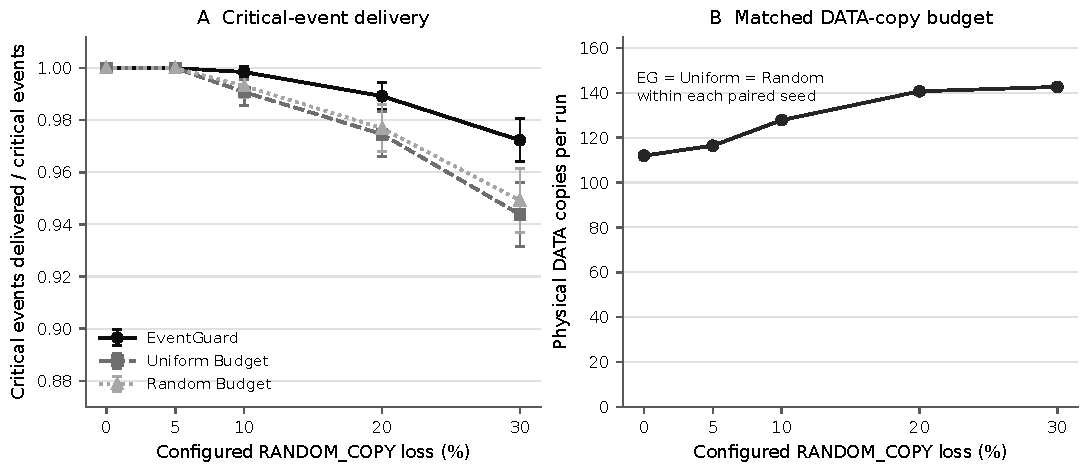
\includegraphics[width=\linewidth]{figures/fig3_exact_budget_host.pdf}
\caption{Exact-budget host comparison under software-injected \texttt{RANDOM\_\allowbreak COPY} loss. Panel A shows mean critical-event delivery ratios (vertical axis displayed from 0.87 to 1.01); Panel B shows mean physical DATA copies per 54-sample run. Error bars are two-sided 95\% Student-t intervals across 100 paired evaluation seeds (31--130). \EG{}, \UB{}, and \RB{} have exactly matched DATA-copy counts within each seed and configured loss rate (0\%, 5\%, 10\%, 20\%, 30\%); the single Panel B series represents all three.}
\label{fig:exact-budget}
\end{figure}

\subsection{Ablation}\label{sec:ablation}

\begingroup\emergencystretch=2em
The host ablation separates importance from link response. At \texttt{RANDOM\_COPY} 20\%, \Ftwo{} delivered 0.9600 of CRITICAL events, versus 0.9892 for both \IO{} and \EG{}; their mean DATA-copy counts were 108.00, 112.00, and 140.68. At 30\%, the three CRITICAL delivery means were 0.9185, 0.9723, and 0.9723; \EG{} used 142.65 copies versus 112.00 for \IO{}. \LO{} delivered 0.942 at 20\% and 0.938 at 30\% in the same host model. These component comparisons are \textbf{not equal-budget tests}. Importance, rather than added link response, accounts for the combined policy's observed CRITICAL-delivery level. The IMPORTANT and overall curves in Fig.~\ref{fig:ablation} show differences between \EG{} and the lower-budget \IO{} rule; this comparison cannot separate extra copies from link-state-aware placement.\par
\endgroup

\begin{figure}[t]
\centering
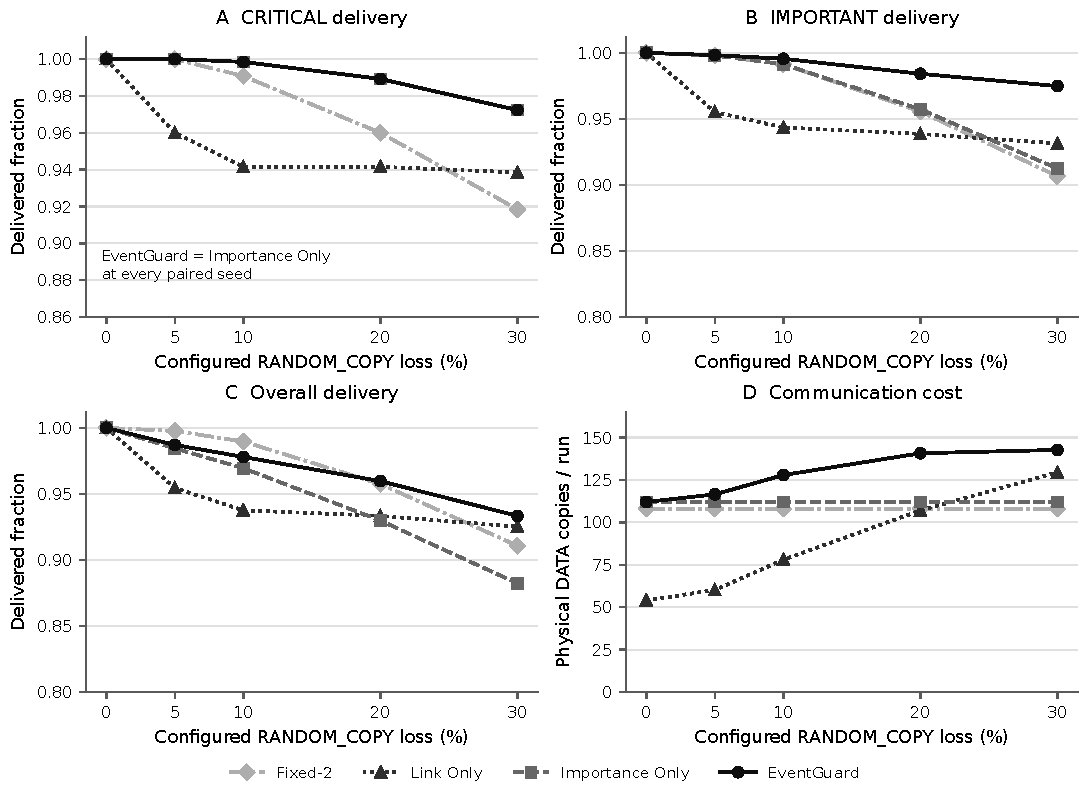
\includegraphics[width=\linewidth]{figures/fig4_ablation_delivery_cost.pdf}
\caption{Host ablation under software-injected \texttt{RANDOM\_COPY} loss. Panels A, B, and C plot mean CRITICAL, IMPORTANT, and overall delivery; Panel D plots mean physical DATA copies per 54-sample run. Each point averages 100 paired evaluation seeds (31--130) for \Ftwo{}, \LO{}, \IO{}, and \EG{}. \EG{} and \IO{} coincide on CRITICAL delivery at every matched seed; their IMPORTANT and overall outcomes and DATA-copy costs can differ. These \EG{}-versus-\IO{} secondary differences are not equal-budget comparisons; the post-hoc IMB diagnostic separately tests placement at a matched DATA-copy budget.}
\label{fig:ablation}
\end{figure}

\subsection{Sensitivity}\label{sec:sensitivity}

Across link-window lengths 8/12/16/24, mean CRITICAL delivery did not change within the reported host conditions, although mean copies and state transitions varied. The CRITICAL-threshold sweep from 2.0 to 4.0 likewise changed copy allocation slightly without changing reported condition-level CRITICAL delivery. Increasing the copy cap from two to three improved host CRITICAL delivery under \texttt{RANDOM\_COPY} (0.9600 to 0.9892 at 20\%; 0.9185 to 0.9723 at 30\%) at greater cost. Under \texttt{BURST\_SAMPLE} at 20\% or 30\%, the cap change left CRITICAL delivery unchanged. No cap-four result exists in frozen v1.

The associated sensitivity visualization is presented as Fig.~\ref{fig:sensitivity} after the hardware cost figure.

\subsection{Real-device execution results}\label{sec:real-device-execution-results}

Table~\ref{tab:hardware-summary} reports means over the six paired hardware seeds. Its displayed ratio is the fraction of ground-truth CRITICAL samples delivered; IMPORTANT and overall ratios are reported immediately below, while copies and bytes are per-run means. Median, standard deviation, confidence interval, and paired statistics remain in the preserved final analysis files. All configured losses were injected in software after reception.

\begin{table}[t]
\centering
\small
\caption{Final 96-run balanced hardware summary (six paired seeds per condition). RC denotes \texttt{RANDOM\_COPY}; BS denotes \texttt{BURST\_SAMPLE}. Critical traffic share uses truth only in retrospective analysis.}
\label{tab:hardware-summary}
\begin{tabular*}{\linewidth}{@{\extracolsep{\fill}}llrrrr@{}}
\toprule
Condition & Strategy & \shortstack{Critical\\delivery} & \shortstack{DATA\\copies} & \shortstack{Total\\bytes} & \shortstack{Critical\\traffic (\%)} \\
\midrule
RC 20\% & \EG{} & 0.9744 & 142.50 & 5,154.5 & 27.4 \\
RC 20\% & \IO{} & 0.9744 & 112.00 & 4,056.0 & 34.8 \\
RC 20\% & \UB{} & 0.9744 & 142.50 & 5,165.3 & 23.0 \\
RC 20\% & \RB{} & 0.9615 & 142.50 & 5,167.5 & 24.1 \\
RC 30\% & \EG{} & 0.9487 & 145.00 & 5,033.2 & 26.9 \\
RC 30\% & \IO{} & 0.9487 & 112.00 & 3,913.0 & 34.8 \\
RC 30\% & \UB{} & 0.9231 & 145.00 & 5,057.0 & 24.0 \\
RC 30\% & \RB{} & 0.9231 & 145.00 & 5,063.5 & 24.0 \\
BS 20\% & \EG{} & 0.7821 & 133.17 & 4,857.7 & 29.3 \\
BS 20\% & \IO{} & 0.7821 & 112.00 & 4,084.2 & 34.8 \\
BS 20\% & \UB{} & 0.7821 & 133.17 & 4,862.0 & 21.1 \\
BS 20\% & \RB{} & 0.7821 & 133.17 & 4,851.2 & 23.9 \\
BS 30\% & \EG{} & 0.7179 & 139.17 & 4,894.5 & 28.1 \\
BS 30\% & \IO{} & 0.7179 & 112.00 & 3,943.3 & 34.8 \\
BS 30\% & \UB{} & 0.7179 & 139.17 & 4,920.5 & 22.7 \\
BS 30\% & \RB{} & 0.7179 & 139.17 & 4,894.5 & 23.9 \\
\bottomrule
\end{tabular*}
\end{table}

The selected hardware \texttt{RANDOM\_COPY} runs reveal the secondary delivery objectives. At 20\%, \EG{} and \IO{} both delivered 0.9744 of CRITICAL events, while IMPORTANT delivery was 0.9885 versus 0.9540 and overall delivery 0.9599 versus 0.9259. \EG{} used 142.50 versus 112.00 DATA copies and 5,154.5 versus 4,056.0 total bytes per run. At 30\%, both strategies delivered 0.9487 of CRITICAL events, while IMPORTANT delivery was 0.9713 versus 0.9253 and overall delivery 0.9259 versus 0.8920; \EG{} used 145.00 versus 112.00 copies and 5,033.2 versus 3,913.0 bytes. Thus the observed \EG{}-minus-\IO{} IMPORTANT gains were 0.0345 and 0.0460, and overall gains were 0.0340 at both rates, with 30.5 and 33.0 extra copies. This hardware comparison changes budget and link-state use together; it cannot attribute the secondary differences to link-state placement. Under \texttt{BURST\_SAMPLE} at both rates, the two strategies had identical CRITICAL, IMPORTANT, and overall delivery while \EG{} used more copies. These are descriptive means across six paired seeds, not confirmatory effect estimates.

All 96 selected runs passed offline checks and showed zero sample-level delivery differences from deterministic host references. This supports faithful execution of the frozen trace, policy, and injected calendar on the device path, not prediction of an uncontrolled radio channel.

\subsection{Exact-budget paired comparisons}\label{sec:exact-budget-paired-comparisons}

\UB{} and \RB{} used exactly \EG{}'s DATA-copy count in every selected condition and seed. \EG{} allocated a larger share of copies to ground-truth CRITICAL samples than either blind allocator in all four conditions (Table~\ref{tab:hardware-summary}). Under \texttt{RANDOM\_COPY} 30\%, \EG{} exceeded each blind baseline in \textbf{two of six} paired seeds and tied four; its mean paired critical-delivery difference was +0.0256 against each. The unadjusted exact Wilcoxon p-value was 0.50 for each, and the exploratory Holm-adjusted value across 12 critical-delivery comparisons was 1.00. Under \texttt{RANDOM\_COPY} 20\%, it tied \UB{} in all six pairs and exceeded \RB{} in one, with a +0.0128 mean difference. Both \texttt{BURST\_SAMPLE} rates yielded six ties against each blind baseline. These sparse differences support targeted allocation and limited condition-specific delivery gains, not confirmatory general superiority. Equal DATA-copy budgets need not produce identical total bytes because ACK activity varies.

\subsection{Pareto tradeoff}\label{sec:pareto-tradeoff}

\IO{} and \EG{} had \textbf{identical CRITICAL delivery in all 24 matched hardware seed/condition pairs}. \EG{} nevertheless used 30.50, 33.00, 21.17, and 27.17 additional DATA copies per run on average in RC 20\%, RC 30\%, BS 20\%, and BS 30\%. Extra total bytes were 1,098.5, 1,120.2, 773.5, and 951.2. For the evaluated CRITICAL-delivery/cost objective, on the empirical within-condition frontier of mean CRITICAL delivery versus DATA copies or bytes, \IO{} appeared in \textbf{4/4} conditions and \EG{} in \textbf{0/4}. These are descriptive frontiers over observed means, not uncertainty regions.

\begin{figure}[t]
\centering
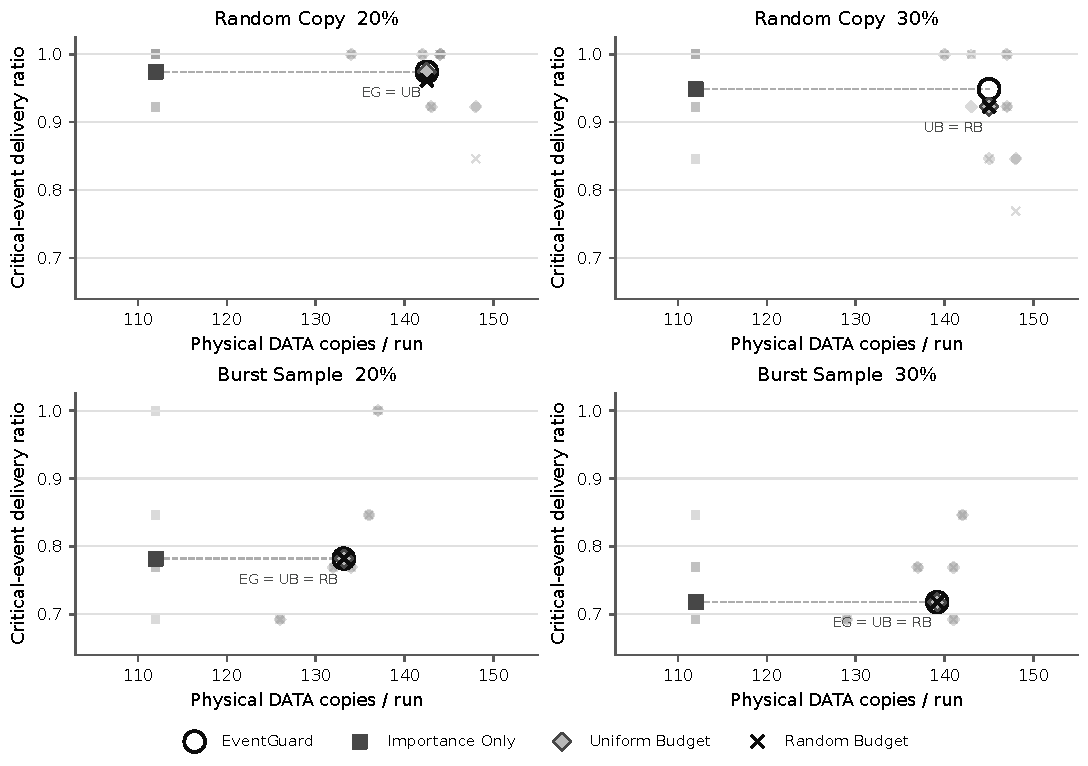
\includegraphics[width=\linewidth]{figures/fig5_hardware_pareto.pdf}
\caption{Real-device critical-event delivery versus DATA-copy cost. Each panel is one configured software-injected loss model/rate; small faint markers show the six preserved seed-level runs (31--36) per strategy, while larger markers show condition means of critical-event delivery and physical DATA copies per 54-sample run. Seed-level points are plotted without jitter. The delivery axis is displayed from 0.64 to 1.025. The 96-run set is a post-hoc balanced prefix from one ESP32-S3/E220 device pair. The dashed horizontal segment connects \IO{} and \EG{} at identical observed mean delivery but different mean copy cost. Coincident event-blind mean points share their exact plotted coordinates. This empirical Pareto display is descriptive, not a significance test or measured RF-loss result.}
\label{fig:hardware-pareto}
\end{figure}

\begin{figure}[t]
\centering
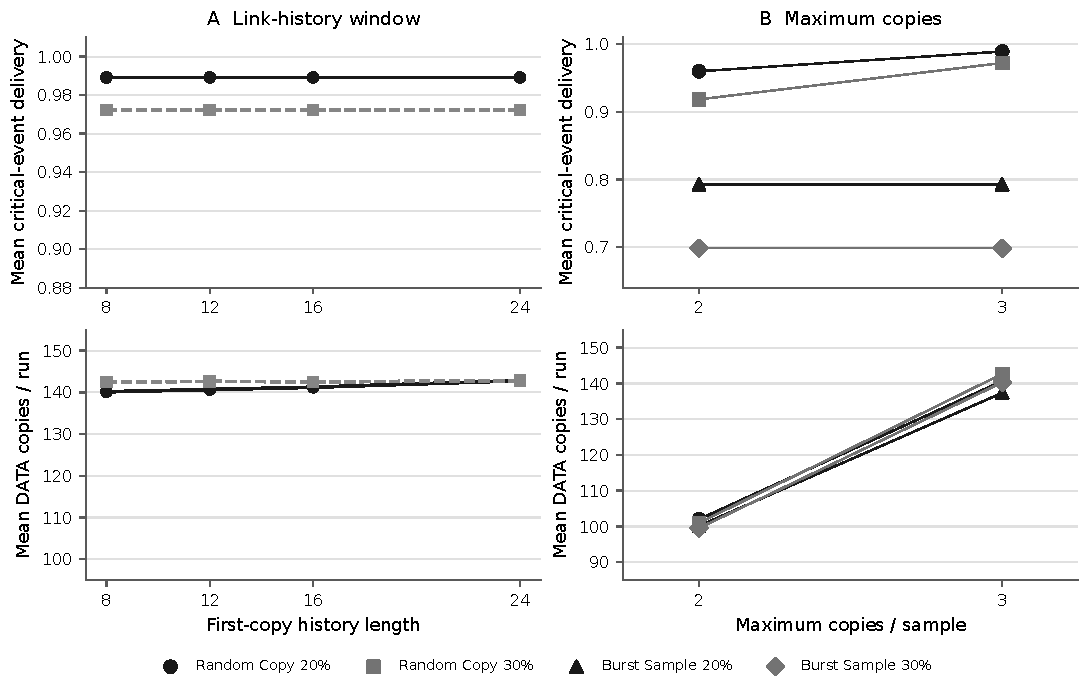
\includegraphics[width=\linewidth]{figures/fig6_sensitivity.pdf}
\caption{Frozen host-only sensitivity under software-injected loss. Left: mean critical-event delivery and physical DATA copies per 54-sample run for first-copy link-history windows 8, 12, 16, and 24 under \texttt{RANDOM\_COPY} at 20\% and 30\%. Right: the same metrics for maximum redundancy 2 versus 3 under \texttt{RANDOM\_COPY} and \texttt{BURST\_SAMPLE} at 20\% and 30\%; thin straight segments connect only the two evaluated cap settings within each condition. Each plotted mean uses 100 evaluation seeds; the segments do not imply intermediate evaluations, and no cap-four result is shown.}
\label{fig:sensitivity}
\end{figure}

\clearpage

\subsection{Post-hoc budget-versus-placement diagnostic}\label{sec:imb-results}

The following results come from the separate 500-run \textbf{host-only, post-hoc} IMB dataset, not the original 8,000-run matrix or the 96 selected hardware runs. The diagnostic was designed after frozen-v1 inspection and before IMB outcome generation; its four primary contrasts are exploratory and were not preregistered. Each row of Table~\ref{tab:imb} uses 100 paired seeds, the same predicted importance, trace, calendar, and exact \EG{} DATA-copy budget. Differences are \EG{} minus IMB; W/T/L counts higher/equal/lower delivery for \EG{}. Holm p-values apply only to this separate four-comparison diagnostic family and are not confirmatory.

\begin{table}[t]
\centering
\small
\caption{Post-hoc importance-matched-budget diagnostic under deterministic, software-injected \texttt{RANDOM\_COPY}. Mean delivery ratios and paired-mean 95\% CIs use 100 seeds. DATA-copy budget is matched in every seed; total bytes may differ with ACK activity.}
\label{tab:imb}
\resizebox{\linewidth}{!}{%
\begin{tabular}{@{}llrrrlrr@{}}
\toprule
Rate & KPI & EG mean & IMB mean & EG--IMB & 95\% CI & W/T/L & Holm p \\
\midrule
RC 20\% & IMPORTANT & 0.984138 & 0.986552 & $-0.002414$ & $[-0.004816,-0.000011]$ & 2/90/8 & 0.367188 \\
RC 20\% & Overall & 0.959630 & 0.957593 & $+0.002037$ & $[-0.001097,+0.005171]$ & 30/54/16 & 0.567222 \\
RC 30\% & IMPORTANT & 0.974828 & 0.975862 & $-0.001034$ & $[-0.002193,+0.000124]$ & 0/97/3 & 0.567222 \\
RC 30\% & Overall & 0.933333 & 0.934259 & $-0.000926$ & $[-0.003816,+0.001964]$ & 21/52/27 & 0.605970 \\
\bottomrule
\end{tabular}%
}
\end{table}

The paired mean differences are small and directionally mixed. Most IMPORTANT pairs tie (90/100 at 20\%, 97/100 at 30\%). The 20\% IMPORTANT paired-mean interval narrowly excludes zero whereas its exact signed-rank and Holm-adjusted descriptive p-values are 0.0918 and 0.3672; sparse, asymmetric differences and different summary assumptions preclude a confirmatory inference. No consistent incremental \EG{} advantage appears over this specific IMB allocator.

The budget-confounded earlier uplift is largely retained by IMB. At RC 20\% IMPORTANT, mean EG--\IO{} / IMB--\IO{} / EG--IMB differences were +0.0269 / +0.0293 / $-0.0024$; for overall delivery, +0.0298 / +0.0278 / +0.0020. At RC 30\% IMPORTANT they were +0.0624 / +0.0634 / $-0.0010$; for overall, +0.0511 / +0.0520 / $-0.0009$. Thus added DATA-copy budget spent with predicted importance is a plausible main explanation for the previous secondary-delivery uplift, not a proof that budget alone explains every difference. All five rate summaries, unadjusted tests, effect sizes, costs, and diagnostic plots remain in the separate repository report.

\section{Separating Importance, Budget, and Link-State Placement}\label{sec:importance-budget-placement}

\subsection{Importance allocation effect}

Against event-blind allocators at an exact per-seed DATA-copy budget, \EG{} directed more traffic to CRITICAL samples and showed small, condition-dependent CRITICAL-delivery gains under \texttt{RANDOM\_COPY}. The constructed \texttt{BURST\_SAMPLE} model erased all copies of affected samples and showed no recovery gain. This supports the role of importance information in deciding where a fixed budget is spent, within these models.

\subsection{Structural saturation of CRITICAL}

The frozen CRITICAL row is 3/3/3 across GOOD, DEGRADED, and BAD, equal to the three-copy cap. Correctly classified CRITICAL samples have no further link-adaptive copy-allocation action; synthetic-benchmark CRITICAL recall was 1.0000. \EG{} and \IO{} matched on CRITICAL delivery in the frozen host matrix and selected hardware pairs. That equality is largely expected from policy structure and does not establish field-classifier accuracy or general link-adaptation failure.

\subsection{Budget explains most secondary uplift}

\EG{} showed higher IMPORTANT and overall delivery than lower-budget \IO{} under \texttt{RANDOM\_COPY} while sending more DATA copies. Because both link-state use and copy budget changed, this original comparison could not isolate placement. IMB retains the same predicted importance and \EG{} budget without link information, reproducing most of the earlier uplift in the 100-seed host diagnostic. The selected hardware secondary gains remain real observations, but their mechanism is not identified by that hardware ablation alone.

\subsection{No consistent incremental placement advantage}

At exact DATA-copy budget and matched trace/calendar, \EG{}-minus-IMB IMPORTANT and overall differences were mixed and close to zero at 20\% and 30\% (Table~\ref{tab:imb}). The post-hoc diagnostic shows no consistent incremental advantage for frozen link-state-aware placement over \textbf{this one} deterministic link-blind, importance-aware allocator under programmed \texttt{RANDOM\_COPY} loss. It does not show that every link-adaptive design is ineffective, that the IMB rule is optimal, or that first-copy ACK history predicts real RF fading. Equal copy budget also leaves small ACK/total-byte differences possible.

\section{Discussion}\label{sec:discussion}

Three distinct mechanisms emerge. \textbf{Importance:} exact-budget event-blind controls show that allocating copies toward CRITICAL samples changes where a fixed budget is spent and can yield limited CRITICAL-delivery gains under independent programmed copy loss. \textbf{Budget:} \EG{} uses more copies than \IO{}; the post-hoc IMB allocator, using the same importance information and \EG{}'s realized budget without link state, reproduces most of the observed IMPORTANT/overall uplift over \IO{}. \textbf{Link-state placement:} \EG{} shows no consistent incremental delivery advantage over this specific IMB rule across the four primary exploratory contrasts. The post-hoc diagnostic therefore weakens any attribution of the earlier IMPORTANT/overall gains specifically to link-state-aware placement.

This decomposition remains bounded. Frozen v1 already saturates correctly classified CRITICAL samples at three copies, making their equality with \IO{} largely structural. The IMB contrast is a host-only, post-hoc comparison against one deterministic, offline counterfactual allocator. It does not prove that extra budget explains all outcomes, that IMB is optimal, or that link adaptation is generally useless. The 96 selected device runs establish execution and deterministic host/firmware agreement, while the preserved incomplete run103 limits broader hardware reliability claims. No measured fading, interference, range, LoRaWAN behavior, or energy efficiency follows from programmed application-layer erasures.

\section{Limitations}\label{sec:limitations}

\begin{table}[t]
\centering
\small
\caption{Scope boundaries and consequences. These bounds apply to all three delivery KPIs and their cost tradeoffs.}
\label{tab:limitations}
\begin{tabularx}{\linewidth}{@{}>{\raggedright\arraybackslash}p{0.40\linewidth}>{\raggedright\arraybackslash}X@{}}
\toprule
Boundary & Consequence for interpretation \\
\midrule
Synthetic, seed-specific 54-sample traces & Limited event diversity; no field-labeled classifier validation \\
One Sensor--Gateway device pair and one topology & No multi-node contention or multi-gateway diversity evidence \\
Deterministic post-reception DATA/ACK injection & Configured 20\%/30\% loss is not measured physical RF PER \\
No controlled fading, interference, or range sweep & No claim about uncontrolled time-varying RF performance \\
UART serialization proxy only & No measured RF PHY airtime, regulatory duty-cycle, or Joule energy result \\
Post-hoc complete prefix, six seeds per condition & Descriptive/exploratory inference; broad population claims unsupported \\
Unresolved seed-37 run103 stall & Hardware reliability outside the selected clean runs remains uncertain \\
Custom E220 application protocol & Results do not characterize LoRaWAN confirmed-message operation \\
Post-hoc IMB host-only counterfactual using EventGuard realized budget & Exploratory, not preregistered or online-deployable; only one deterministic link-blind allocation rule is tested \\
\bottomrule
\end{tabularx}
\end{table}

Seed-level replication cannot substitute for independent device pairs, antennas, placements, interference regimes, or measured channel histories. The classifier uses designed synthetic labels; its confusion matrix is not a field accuracy estimate. No multi-node traffic contention, multi-gateway reception, current draw, regulatory duty-cycle, or measured physical packet-error rate was evaluated. The earlier v0 pilot remains separate because its shorter trace and design cannot be pooled with frozen v1. IMB is also separate from \texttt{v1.0.0}: it uses no hardware, cannot establish superiority against every importance-aware allocator, and does not measure RF-channel prediction.

\section{Future Work}\label{sec:future-work}

A prospective, preregistered matched-budget link-state study could compare a fixed importance-aware link-blind rule with a link-aware policy under controlled, time-varying RF conditions. Such a study should measure physical DATA/ACK reception, available RSSI/SNR or another link observable, packet-error rate, unplanned errors, current draw, and RF airtime across multiple device pairs. A separately specified policy would need actual CRITICAL action space before testing CRITICAL link adaptation, with a renewed canonical calendar and Python/C parity. Field-labeled events, multi-node contention, and multi-gateway diversity remain open. These are new studies, not an instruction to fill the interrupted Stage 1 matrix or immediately run IMB on hardware.

\section{Conclusion}\label{sec:conclusion}

Frozen \EG{}-v1 combines event importance, additional transmission budget under degraded link estimates, and link-state-aware copy placement. Exact-budget event-blind controls support importance-aware allocation for CRITICAL traffic under some independent programmed-loss conditions. Correctly classified CRITICAL samples are structurally saturated at the three-copy cap, so \EG{} and \IO{} match on their CRITICAL delivery. Their IMPORTANT/overall comparison is budget-confounded: \EG{} spends more copies. A separate post-hoc, host-only IMB diagnostic reproduced most of the earlier IMPORTANT/overall uplift without link state. Across four primary exploratory contrasts, \EG{} showed mixed, near-zero differences relative to IMB. The current evidence supports importance information and added DATA-copy budget as the main contributors while providing no consistent incremental placement advantage over this specific link-blind baseline under deterministic software-injected \texttt{RANDOM\_COPY} loss.

These results do not establish general link-adaptation inefficacy or measured RF reliability. Prospective matched-budget comparisons and real time-varying RF validation remain future work.

\section*{Data and Code Availability}

\begingroup\emergencystretch=3em
The public \href{https://github.com/Sver0411/EventGuard-LoRa}{EventGuard-LoRa repository} and frozen \texttt{v1.0.0} release provide the algorithm specification, source code, archived experimental manifests and raw logs, analysis scripts, and identifiers for the selected 96-run hardware dataset. The README and final hardware analysis files give offline reproduction commands. The finalizer regenerates the audit and descriptive statistics from preserved records without accessing devices. Additional post-hoc IMB materials---the protocol, 500 host-only runs, paired tests, report, plots, and provenance---are provided separately in \path{results/posthoc_importance_matched_budget/}; they are not part of the original frozen \texttt{v1.0.0} dataset. Public access supports inspection and citation. Reuse permissions are described in the repository's \texttt{NOTICE.md}.\par
\endgroup

\bibliographystyle{unsrt}
\bibliography{references}
\end{document}
